\documentclass[a4paper,11pt]{article}
\usepackage{amsmath,amsthm,amsfonts,amssymb,amscd,amstext,vmargin,graphics,graphicx,tabularx,multicol} \usepackage[french]{babel}
\usepackage[utf8]{inputenc}  
\usepackage[T1]{fontenc} 
\usepackage[T1]{fontenc}
\usepackage{amsmath,amssymb}
\usepackage{pstricks-add,tikz,tkz-tab,variations}
\usepackage[autolanguage,np]{numprint} 
\usepackage{color}
\usepackage{ulem}

\setmarginsrb{1.5cm}{0.5cm}{1cm}{0.5cm}{0cm}{0cm}{0cm}{0cm} %Gauche, haut, droite, haut
\newcounter{numexo}
\newcommand{\exo}[1]{\stepcounter{numexo}\noindent{\bf Exercice~\thenumexo} : \marginpar{\hfill /#1}}
\reversemarginpar


\newcounter{enumtabi}
\newcounter{enumtaba}
\newcommand{\q}{\stepcounter{enumtabi} \theenumtabi.  }
\newcommand{\qa}{\stepcounter{enumtaba} (\alph{enumtaba}) }
\newcommand{\initq}{\setcounter{enumtabi}{0}}
\newcommand{\initqa}{\setcounter{enumtaba}{0}}

\newcommand{\be}{\begin{enumerate}}
\newcommand{\ee}{\end{enumerate}}
\newcommand{\bi}{\begin{itemize}}
\newcommand{\ei}{\end{itemize}}
\newcommand{\bp}{\begin{pspicture*}}
\newcommand{\ep}{\end{pspicture*}}
\newcommand{\bt}{\begin{tabular}}
\newcommand{\et}{\end{tabular}}
\renewcommand{\tabularxcolumn}[1]{>{\centering}m{#1}} %(colonne m{} centrée, au lieu de p par défault) 
\newcommand{\tnl}{\tabularnewline}

\newcommand{\trait}{\noindent \rule{\linewidth}{0.2mm}}
\newcommand{\hs}[1]{\hspace{#1}}
\newcommand{\vs}[1]{\vspace{#1}}

\newcommand{\N}{\mathbb{N}}
\newcommand{\Z}{\mathbb{Z}}
\newcommand{\R}{\mathbb{R}}
\newcommand{\C}{\mathbb{C}}
\newcommand{\Dcal}{\mathcal{D}}
\newcommand{\Ccal}{\mathcal{C}}
\newcommand{\mc}{\mathcal}

\newcommand{\vect}[1]{\overrightarrow{#1}}
\newcommand{\ds}{\displaystyle}
\newcommand{\eq}{\quad \Leftrightarrow \quad}
\newcommand{\vecti}{\vec{\imath}}
\newcommand{\vectj}{\vec{\jmath}}
\newcommand{\Oij}{(O;\vec{\imath}, \vec{\jmath})}
\newcommand{\OIJ}{(O;I,J)}

\newcommand{\bmul}[1]{\begin{multicols}{#1}}
\newcommand{\emul}{\end{multicols}}


\newcommand{\reponse}[1][1]{%
\multido{}{#1}{\makebox[\linewidth]{\rule[0pt]{0pt}{20pt}\dotfill}
}}

\newcommand{\titre}[5] 
% #1: titre #2: haut gauche #3: bas gauche #4: haut droite #5: bas droite
{
\noindent #2 \hfill #4 \\
#3 \hfill #5

\vspace{-1.6cm}

\begin{center}\rule{6cm}{0.5mm}\end{center}
\vspace{0.2cm}
\begin{center}{\large{\textbf{#1}}}\end{center}
\begin{center}\rule{6cm}{0.5mm}\end{center}
}



\begin{document}
\pagestyle{empty}
\titre{Contrôle : Statistiques}{Nom}{Prénom}{Date}{Classe}
\vspace*{1cm}


\exo{4} Voici les points d'Adil et Léo au lancer de dés.\\

\textbf{Adil :} 6 ; 5 ; 1 ; 3 ; 4 ; 1 ; 2 ; 5 ; 4 ; 3 ; 4.\\



\textbf{Léo :} \hspace*{1.5cm} \begin{tabular}{|c|c|c|c|c|c|c|}
\hline 
\textbf{Nombre de points} & 1 & 2 & 3 & 4 & 5 & 6 \\ 
\hline 
\textbf{Effectif} & 0 & 3 & 2 & 2 & 1 & 2 \\ 
\hline 
\end{tabular} 


\vspace*{1cm}

\initq \noindent \q Déterminer la médiane de la série d'Adil. Interpréter cette médiane pour la situation.\\
\q Déterminer la médiane de la série de Léo. Interpréter cette médiane pour la situation.\\
\q Celui qui obtient la médiane la plus élevée gagne la partie. Qui a gagné cette partie?\\

\vspace*{1cm}


\exo{3} Cet histogramme donne la répartition, selon l'âge, des 37 enfants inscrits à un centre de loisirs.\\

\includegraphics[scale=0.7]{statgraph.eps} \\

\noindent \initq \q Calculer l'étendue de cette série statistique.\\
\q Déterminer l'âge médian de ce centre de loisirs. Interpréter votre résultat.\\



\vspace*{1cm}

\exo{6} Voici les résultats d'une enquête auprès des 30 élèves d'une classe de troisième sur le nombre de décorations d'halloween qu'ils ont dans leur foyer.\\

\begin{tabular}{|c|c|c|c|c|c|c|}
\hline 
\textbf{Nombres de décorations} & 14 & 15 & 18 & 20 & 23 & 24 \\ 
\hline 
\textbf{Effectif} & 5 & 3 & 3 & 4 & 7 & 8 \\ 
\hline 
\end{tabular} 




\vspace*{0.5cm}

\initq 
\noindent \q Calculer l'étendue de cette série statistique.\\
\q Déterminer la moyenne de cette série statistique. \textit{Interpréter le résultat.}\\
\q Calculer le pourcentage d'élèves  qui ont plus de 21 décorations dans leur foyer.\\
\q Un nouvel élève arrive  dans cette classe. Il n'a malheureusement aucune décoration chez lui.\\
Que deviennent alors la moyenne ?\\	

\newpage

\vspace*{1cm}

\exo{7}

Dans tout l'exercice, on étudie les performances réalisées par les athlètes qui ont participé aux finales du 100 m masculin des Jeux Olympiques de 2016 et de 2012.\\
On donne ci-dessous des informations sur les temps mis par les athlètes pour parcourir 100 m.\\

\textbf{Finale du 100 m aux Jeux Olympiques de 2016 :}\\
Temps réalisés par tous les finalistes :\\
\includegraphics[scale=0.8]{100m.eps} \\

\textbf{Finale du 100 m aux Jeux Olympiques de 2012 :}\\
\includegraphics[scale=0.8]{100mbis.eps} \\

\initq
\noindent \q Quel est le temps du vainqueur de la finale en 2016 ?\\
\q Lors de quelle finale la moyenne des temps pour effectuer 100 m est-elle la plus petite ?\\
\q Lors de quelle finale le meilleur temps a-t-il été réalisé ?\\
\q L'affirmation suivante est-elle vraie ou fausse ?\\
\textbf{Affirmation} : « Seulement trois athlètes ont mis moins de 10 s à parcourir les 100 m de la finale
de 2012 ».\\


\end{document}
